\documentclass[aspectratio=169,11pt]{beamer}
\usetheme{default}
\usepackage[T1]{fontenc}
\usepackage{amsmath,amssymb,booktabs,graphicx,tikz}
\usetikzlibrary{positioning,arrows.meta,shapes.misc}

\definecolor{ink}{HTML}{1B2430}
\definecolor{ink2}{HTML}{4A5462}
\definecolor{paper}{HTML}{F7F6F2}
\definecolor{trace}{HTML}{2A78D6}
\definecolor{image}{HTML}{C9551F}
\definecolor{model}{HTML}{13865D}
\definecolor{problem}{HTML}{B3372E}
\definecolor{soft}{HTML}{ECEAE3}

\setbeamercolor{background canvas}{bg=paper}
\setbeamercolor{normal text}{fg=ink}
\setbeamercolor{frametitle}{fg=ink}
\setbeamercolor{structure}{fg=trace}
\setbeamerfont{frametitle}{size=\Large,series=\bfseries}
\setbeamertemplate{navigation symbols}{}
\setbeamertemplate{itemize items}[circle]
\setbeamertemplate{footline}{\hfill\textcolor{ink2}{\scriptsize ccd\_opt\_ml \textperiodcentered{} level 1 overview \textperiodcentered{} \insertframenumber}\hspace{1em}\vspace{0.6em}}
\setbeamersize{text margin left=1.2cm,text margin right=1.2cm}

\newcommand{\eyebrow}[2][trace]{{\color{#1}\scriptsize\bfseries\MakeUppercase{#2}}\par\vspace{0.2em}}
\newcommand{\fig}[2][\textwidth]{\includegraphics[width=#1,height=#2,keepaspectratio]}
\tikzset{
  box/.style={draw=#1,fill=#1!8,rounded corners=3pt,align=center,font=\footnotesize,minimum height=1.1cm,text width=2.1cm,line width=0.8pt},
  box/.default=ink2,
  arr/.style={-{Stealth[length=2.5mm]},line width=0.9pt,color=ink2},
  s/.style={box=#1,text width=1.55cm,minimum height=0.9cm,font=\scriptsize}, s/.default=ink2,
}
\newcommand{\divider}[3]{%
{\setbeamercolor{background canvas}{bg=ink}\setbeamertemplate{footline}{}
\begin{frame}[plain]
\vfill
{\color{#3}\small\bfseries\MakeUppercase{#1}}\par\vspace{0.6em}
{\color{paper}\huge\bfseries #2}\par\vspace{1em}
\vfill
\end{frame}}}

\title{Can a two-second trace predict what a ten-minute image will show?}
\subtitle{ccd\_opt\_ml, level 1: skipper-CCD read noise, dark charge and gain from short readout traces}
\date{PA03 \textperiodcentered{} board 101 \textperiodcentered{} 43 packets of 2026-11-02/03 \textperiodcentered{} analyses up to 2026-11-04}

\begin{document}

{\setbeamercolor{background canvas}{bg=ink}\setbeamertemplate{footline}{}
\begin{frame}[plain]
\vfill
{\color{trace!60}\small\bfseries CCD\_OPT\_ML \textperiodcentered{} LEVEL 1}\par\vspace{0.8em}
{\color{paper}\LARGE\bfseries Can a two-second trace predict what a ten-minute image will show?}\par\vspace{1em}
{\color{paper!75}\normalsize The pipeline, the models with their math, the first real data, and what carries over to other CCDs.}\par\vfill
{\color{paper!75}\small PA03 \textperiodcentered{} board 101 (acm101) \textperiodcentered{} 43 packets taken 2026-11-02/03 \textperiodcentered{} analyses up to 2026-11-04}\par\vspace{0.5em}
{\small\colorbox{trace}{\color{paper} trace}\ \colorbox{image}{\color{paper} image}\ \colorbox{model}{\color{paper} model}\ \colorbox{problem}{\color{paper} problem}}
\end{frame}}

% ============================================================================================================
\begin{frame}{Tuning a CCD means trying settings, and every try costs an image}
\eyebrow{The goal}
\begin{columns}[T]
\column{0.32\textwidth}
{\color{image}\bfseries IMAGE}\par{\Large\bfseries $\sim$5--10 min}\par\small 16 rows $\times$ 1000 columns $\times$ 500 skips. run\_WADERs gives the truth: $\sigma_e$, $\lambda$, gain.
\column{0.32\textwidth}
{\color{trace}\bfseries TRACE}\par{\Large\bfseries $\sim$2 s}\par\small $2\times5$ pixels $\times$ 500 skips, every raw ADC sample kept.
\column{0.32\textwidth}
{\color{model}\bfseries LEVEL-1 QUESTION}\par\normalsize\bfseries Does the trace already tell us what the image will show?\par\mdseries\small If yes: scan settings with traces, image only the best.
\end{columns}
\vspace{1.2em}
\begin{center}
\resizebox{\textwidth}{!}{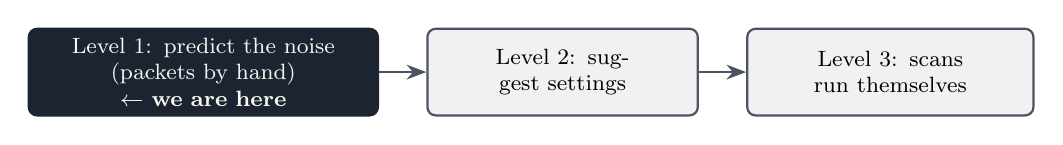
\begin{tikzpicture}[node distance=0.6cm]
\node[box=ink,text width=4.2cm,fill=ink,text=paper] (l1) {Level 1: predict the noise\\(packets by hand) \textbf{$\leftarrow$ we are here}};
\node[box,right=of l1,text width=3.2cm] (l2) {Level 2: suggest settings};
\node[box,right=of l2,text width=3.4cm] (l3) {Level 3: scans run themselves};
\draw[arr] (l1)--(l2); \draw[arr] (l2)--(l3);
\end{tikzpicture}}
\end{center}
\end{frame}

\begin{frame}{A skipper CCD measures each pixel's charge $N$ times and averages}
\eyebrow{The physics}
\begin{columns}[T]
\column{0.55\textwidth}
The charge is moved back and forth under the sense node without being destroyed. Each \textbf{skip} is one measurement; averaging $N=500$ skips beats down the read noise until slow noise sets a floor:
\[
\sigma_{\rm ADU}^2(N)=\frac{\sigma_1^2}{N}+\sigma_{\rm floor}^2,\qquad \sigma_e=\frac{\sigma_{\rm ADU}}{g}.
\]
Here $\sigma_1\approx5.6$ ADU, so $5.6/\sqrt{500}=0.25$ ADU $\approx0.19\,e^-$ at $g=1.3$.
\column{0.42\textwidth}
\begin{itemize}\small
\item {\color{image}\bfseries $\sigma_e$}: read noise (e$^-$), width of the 0-electron peak; 0.15--0.19 here
\item {\color{image}\bfseries $\lambda$}: dark charge (e$^-$/pixel): dark current while rows wait + clock-induced charge (CIC)
\item {\color{image}\bfseries $g$}: gain (ADU/e$^-$), spacing of the electron peaks; 1.26--1.34
\end{itemize}
\end{columns}
\end{frame}

\begin{frame}{A trace is the raw waveform of 10 pixels, every ADC sample kept}
\eyebrow{The input}
\begin{columns}[c]
\column{0.64\textwidth}\fig{0.72\textheight}{figures/reuse_t_trace_anatomy.png}
\column{0.34\textwidth}\small
\textbf{Each skip:} a pedestal window, the charge is dumped, a signal window.\par\medskip
\textbf{CDS} = signal $-$ pedestal: one number per skip, 500 per pixel.\par\medskip
The image keeps only the pixel \emph{averages}; the trace keeps the whole waveform, so we can see \emph{why} the noise is what it is.
\end{columns}
\end{frame}

\begin{frame}{Every trace becomes 141 numbers and 16 curves}
\eyebrow{From a trace to numbers}
\begin{columns}[T]
\column{0.58\textwidth}
\fig{0.48\textheight}{figures/reuse_t_trace_noise.png}\par
The Allan curve is fitted as
\[\sigma_A^2(n)=\frac{a^2}{n}+b^2,\qquad a=\sigma_1,\ b=\sigma_{\rm floor}.\]
\column{0.40\textwidth}\small
\textbf{Feature groups} (src/trace\_features.py)
\begin{itemize}\footnotesize
\item \textbf{noise}: CDS $\sigma$, white noise per skip, Allan / Hadamard at $n=50$, 1/f corner, band powers
\item \textbf{skip}: first-skip excess, ringing in skips 1--4, droop
\item \textbf{edge}: reset pulse and SW dip shape, jitter, recovery
\item \textbf{slow / start / clock}: row-start recovery, drifts, clock pickup
\item \textbf{curves}: Allan, spectra, mean skip shape, start transient (256 points each)
\end{itemize}
\end{columns}
\end{frame}

% ============================================================================================================
\divider{Part 2}{From the DAQ to a training table}{trace!60}

\begin{frame}{A packet: reference traces, one change, new traces, one image}
\eyebrow{The unit of data}
\begin{center}
\resizebox{\textwidth}{!}{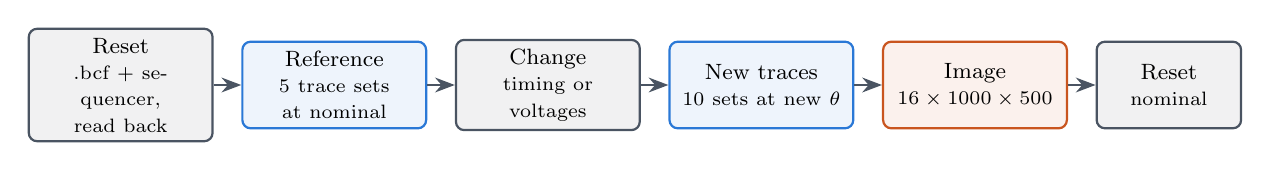
\begin{tikzpicture}[node distance=0.35cm]
\node[box] (a) {Reset\\\scriptsize .bcf + sequencer, read back};
\node[box=trace,right=of a] (b) {Reference\\\scriptsize 5 trace sets at nominal};
\node[box,right=of b] (c) {Change\\\scriptsize timing or voltages};
\node[box=trace,right=of c] (d) {New traces\\\scriptsize 10 sets at new $\theta$};
\node[box=image,right=of d] (e) {Image\\\scriptsize $16\times1000\times500$};
\node[box,right=of e,text width=1.6cm] (f) {Reset\\\scriptsize nominal};
\foreach \x/\y in {a/b,b/c,c/d,d/e,e/f} \draw[arr] (\x)--(\y);
\end{tikzpicture}}
\end{center}
\vspace{0.8em}
\begin{columns}[T]
\column{0.32\textwidth}\small\textbf{Session A \textperiodcentered{} 14 packets}\par timing: integration time, H-clock and RG delays, one at a time
\column{0.32\textwidth}\small\textbf{Session B \textperiodcentered{} 18 packets}\par voltages: VDD, VR, VSUB, clock rails, one at a time
\column{0.32\textwidth}\small\textbf{Session C \textperiodcentered{} 11 packets}\par several knobs at once: the held-out test
\end{columns}
\vspace{1em}
\textbf{1 packet = 4 amplifiers = 4 training rows.} The models are never told which amplifier a row is. Only board 101's settings were changed.
\end{frame}

\begin{frame}{Every packet starts from a verified nominal state}
\eyebrow{Taking packets safely}
\begin{columns}[T]
\column{0.32\textwidth}
{\color{trace}\bfseries Reset both halves}\par\small The .bcf sets the voltages; the \textbf{sequencer} holds the clock timing. nominal() restores both and reloads the sequencer.
\column{0.32\textwidth}
{\color{model}\bfseries Read it back}\par\small Biases within 0.3 V, offsets and rails within 0.05 V, every delay and the sequencer name checked. Anything off: ``NOT NOMINAL'', the packet stops.
\column{0.32\textwidth}
{\color{problem}\bfseries Catch damaged traces}\par\small check\_trace\_files.py decodes each trace on the spot; damaged ones are retaken; more than 5 restarts the packet (v2).
\end{columns}
\vspace{1.5em}
\colorbox{soft}{\parbox{0.95\textwidth}{\small\textbf{First night:} all 43 packets started at nominal and every requested change arrived; 2370 of 2580 board-101 traces usable (8\,\% damaged).}}
\end{frame}

\begin{frame}{One command turns a packet into training rows}
\eyebrow{Processing}
\begin{center}
\resizebox{\textwidth}{!}{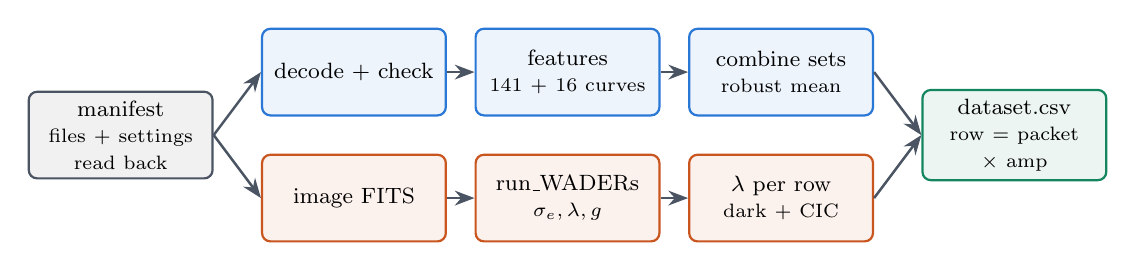
\begin{tikzpicture}[node distance=0.35cm and 0.35cm]
\node[box] (m) {manifest\\\scriptsize files + settings read back};
\node[box=trace,right=0.6cm of m,yshift=0.8cm] (t1) {decode + check};
\node[box=trace,right=of t1] (t2) {features\\\scriptsize 141 + 16 curves};
\node[box=trace,right=of t2] (t3) {combine sets\\\scriptsize robust mean};
\node[box=image,right=0.6cm of m,yshift=-0.8cm] (i1) {image FITS};
\node[box=image,right=of i1] (i2) {run\_WADERs\\\scriptsize $\sigma_e,\lambda,g$};
\node[box=image,right=of i2] (i3) {$\lambda$ per row\\\scriptsize dark + CIC};
\node[box=model,right=0.6cm of t3,yshift=-0.8cm] (ds) {dataset.csv\\\scriptsize row = packet $\times$ amp};
\draw[arr] (m.east)--(t1.west); \draw[arr] (m.east)--(i1.west);
\draw[arr] (t1)--(t2); \draw[arr] (t2)--(t3); \draw[arr] (i1)--(i2); \draw[arr] (i2)--(i3);
\draw[arr] (t3.east)--(ds.west); \draw[arr] (i3.east)--(ds.west);
\end{tikzpicture}}
\end{center}
\vspace{0.5em}
\begin{itemize}\small
\item \textbf{model\_inputs/}: one file per model family (features, curves, physics, sets, pretrain = every unlabelled trace).
\item \textbf{trace\_ok rule}: a row without one usable trace at its own settings is not used (L1\_37, 40, 41 lost all 40).
\end{itemize}
\end{frame}

\begin{frame}{run\_WADERs fits the pixel values as a comb of electron peaks}
\eyebrow[image]{The labels}
\begin{columns}[T]
\column{0.5\textwidth}
\[p(x)=\sum_{k=0}^{\infty}\mathrm{Pois}(k;\lambda)\ \mathcal N\!\left(x;\ \mu+k\,g,\ \sigma^2\right)\]
\small A pixel holds $k$ electrons with probability $\mathrm{Pois}(k;\lambda)$; its average sits at $\mu+kg$, blurred by $\sigma$. The fit gives $\lambda$, $g$ and $\sigma_e=\sigma/g$.
\[\lambda_r=\mathrm{CIC}+\mathrm{DC}\cdot t_r\]
Row by row, $\lambda$ grows with the wait $t_r$: slope = dark current, intercept = CIC.
\column{0.48\textwidth}
\fig{0.36\textheight}{figures/reuse_guide_rows.png}\par\medskip
{\footnotesize\begin{tabular}{lccc}\toprule
repeat at nominal & $\sigma_e$ & $\lambda$ & gain\\\midrule
label scatter & 2.2\,\% & 11\,\% & 0.6\,\%\\\bottomrule
\end{tabular}}\par\smallskip
\footnotesize No model can be judged below the label scatter; $\lambda$'s is large because it drifted $\sim$20\,\% over the night.
\end{columns}
\end{frame}

\begin{frame}{The row-start drift correction helped in October and hurt in November}
\eyebrow[problem]{A label problem, found and fixed}
\fig{0.42\textheight}{figures/reuse_s2_drift_profile.png}
\begin{columns}[T]
\column{0.32\textwidth}\small{\color{model}\bfseries October}\par the 0-e$^-$ level sagged $-1$ ADU at every row start; the correction took $\chi^2$/ndf 2.7--5.1 $\to$ 0.65--1.15
\column{0.32\textwidth}\small{\color{problem}\bfseries November}\par raw images already fit well (0.8--1.3); the correction inflated session-A $\sigma_e$ up to $\times3$ and raised $\lambda$ 7--10\,\%
\column{0.32\textwidth}\small{\color{trace}\bfseries Decision}\par correction off; labels checked against replicates (L1\_06 / L1\_23: 0.145 / 0.144 e$^-$)
\end{columns}
\end{frame}

\begin{frame}{Feature tiers, decided without looking at a single label}
\eyebrow{Which features to give the models}
\begin{columns}[T]
\column{0.45\textwidth}\small
From the traces alone (lvl1/feature\_study.py), each feature gets evidence scores:
\begin{itemize}\small
\item does it \textbf{respond to the settings}? (F-test across packets)
\item does it \textbf{repeat} at the same setting?
\item is it \textbf{redundant} with a better one?
\end{itemize}
Tiers frozen in git (b7d25ca) before any training. Each model's best set is chosen by A+B cross-validation, per target.
\column{0.52\textwidth}
{\small\begin{tabular}{llp{3.3cm}}\toprule
set & features & what is in it\\\midrule
none & 0 & settings only\\
P & 8 & protected noise estimators\\
P+A1 & 44 & + strongest evidence\\
P+A & 81 & + good evidence\\
P+A+B & 96 & + weaker evidence\\
all & 141 & everything\\\bottomrule
\end{tabular}}
\end{columns}
\end{frame}

% ============================================================================================================
\divider{Part 3}{The models, and how we test them}{model!60}

\begin{frame}{Predict three log labels per amplifier from settings and traces}
\eyebrow[model]{The learning problem}
\[
y_i=\left(\log\sigma_{e,i},\ \log\lambda_i,\ \log g_i\right),\qquad
\mathrm{error}=100\sqrt{\tfrac1n\textstyle\sum_i(\hat y_i-y_i)^2}\ \%
\]
\begin{columns}[T]
\column{0.24\textwidth}\small\textbf{$\theta$ settings}\par 67 numbers: delays, clock rails, biases
\column{0.24\textwidth}\small{\color{trace}\textbf{$u$ own trace}}\par features of this amplifier's traces at $\theta$
\column{0.24\textwidth}\small{\color{trace}\textbf{$v$ reference}}\par same features at nominal, minutes earlier
\column{0.24\textwidth}\small{\color{trace}\textbf{$s$ packet state}}\par $s_i=\tfrac{1}{|p|}\sum_{j\in p}(v_j-\bar v_{a(j)})$
\end{columns}
\vspace{1em}
\small Log space makes the error a \textbf{relative} error and turns $\sigma_e=\sigma_{\rm ADU}/g$ into a sum. No trace model sees the amplifier's name; three references do, to measure what that name is worth.
\end{frame}

\begin{frame}{Seventeen models in four families}
\eyebrow[model]{The model map}
\begin{columns}[T]
\column{0.48\textwidth}
\colorbox{soft}{\parbox{0.95\textwidth}{\small\textbf{Baselines and references (no trace)}\par\footnotesize mean (training average) \textperiodcentered{} settings (GP on $\theta$) \textperiodcentered{} settings\_amp, settings\_amp\_trees (GP / boosted trees on $\theta$ + the amplifier's name)}}\par\medskip
\colorbox{trace!10}{\parbox{0.95\textwidth}{\small\textbf{On trace curves}\par\footnotesize cnn (1-D convolutions) \textperiodcentered{} pretrained (encoder pre-trained on unlabelled traces, fine-tuned) \textperiodcentered{} deep\_kernel (GP on that encoder's output)}}
\column{0.48\textwidth}
\colorbox{trace!10}{\parbox{0.95\textwidth}{\small\textbf{On trace features $[\theta;u;v]$}\par\footnotesize ridge (Bayesian linear) \textperiodcentered{} trees (boosted) \textperiodcentered{} gp (free length scales) \textperiodcentered{} gp\_dim (dimension-scaled prior) \textperiodcentered{} nn (network ensemble)}}\par\medskip
\colorbox{model!10}{\parbox{0.95\textwidth}{\small\textbf{Physics-structured}\par\footnotesize physics (Allan term) \textperiodcentered{} physics\_white (white-noise term) \textperiodcentered{} physics\_joint (dark + CIC) \textperiodcentered{} sets (learned set combiner) \textperiodcentered{} physics\_hier (told the amplifier)}}
\end{columns}
\end{frame}

\begin{frame}{A GP predicts by weighting training rows by how similar they are}
\eyebrow[model]{Gaussian processes \textperiodcentered{} settings, settings\_amp, gp, gp\_dim}
\small
\[
y=f(x)+\varepsilon,\quad f\sim\mathcal{GP}(0,k),\quad k(x,x')=c\left(1+\sqrt5r+\tfrac53r^2\right)e^{-\sqrt5r},\quad r^2=\sum_j\frac{(x_j-x'_j)^2}{\ell_j^2}
\]
\[
\hat y_*=\mathbf k_*^\top(K+\sigma_n^2I)^{-1}\mathbf y,\qquad \max_\phi\ \log p(\mathbf y|\phi)=-\tfrac12\mathbf y^\top K_y^{-1}\mathbf y-\tfrac12\log|K_y|-\tfrac n2\log2\pi
\]
\begin{columns}[c]
\column{0.56\textwidth}\fig{0.3\textheight}{figures/reuse_guide_gp.png}
\column{0.42\textwidth}\footnotesize
$1/\ell_j$ = how much input $j$ matters (ARD relevance).\par
\textbf{gp}: no prior (box bounds) \textperiodcentered{} \textbf{gp\_dim}: $\ell_j\sim\mathrm{LogNormal}(\sqrt2+\tfrac12\log d,\sqrt3)$ \textperiodcentered{} \textbf{SAAS}: $\tau\sim\mathrm{HC}(0.1)$, $1/\ell_j^2\sim\mathrm{HC}(\tau)$, switches inputs off unless needed (used for $\lambda$).
\end{columns}
\end{frame}

\begin{frame}{Boosted trees add up hundreds of small step functions}
\eyebrow[model]{Boosted trees and ridge}
\small
\[F_0=\bar y,\qquad F_m(x)=F_{m-1}(x)+\nu\,h_m(x),\qquad h_m\ \text{fit to}\ r_i=y_i-F_{m-1}(x_i),\quad \nu=0.05\]
\fig{0.32\textheight}{figures/reuse_guide_trees.png}
\begin{columns}[T]
\column{0.32\textwidth}\footnotesize\textbf{300 trees}, $\le15$ leaves, $\ge10$ rows per leaf; error bars from 16\,\% / 84\,\% quantile models
\column{0.32\textwidth}\footnotesize{\color{problem}\textbf{The 10-row catch:}} a knob changed in only 1--2 packets (4--8 rows) can never be split on
\column{0.32\textwidth}\footnotesize\textbf{ridge:} $y=b+w^\top\tilde x$, $w\sim\mathcal N(0,\lambda_w^{-1}I)$, precisions by maximizing the evidence
\end{columns}
\end{frame}

\begin{frame}{Networks learn their own features from the curves}
\eyebrow[model]{nn, cnn, pretrained, deep\_kernel}
\begin{center}
\resizebox{\textwidth}{!}{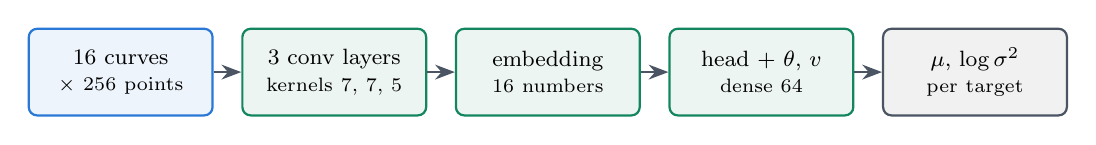
\begin{tikzpicture}[node distance=0.35cm]
\node[box=trace] (a) {16 curves\\\scriptsize $\times$ 256 points};
\node[box=model,right=of a] (b) {3 conv layers\\\scriptsize kernels 7, 7, 5};
\node[box=model,right=of b] (c) {embedding\\\scriptsize 16 numbers};
\node[box=model,right=of c] (d) {head + $\theta$, $v$\\\scriptsize dense 64};
\node[box,right=of d] (e) {$\mu$, $\log\sigma^2$\\\scriptsize per target};
\foreach \x/\y in {a/b,b/c,c/d,d/e} \draw[arr] (\x)--(\y);
\end{tikzpicture}}
\end{center}
\[
\mathcal L=\tfrac12\left[\log\sigma^2(x)+\frac{(y-\mu(x))^2}{\sigma^2(x)}\right],\qquad
\hat\mu=\tfrac1K\textstyle\sum_k\mu_k,\quad \hat\sigma^2=\tfrac1K\sum_k\sigma_k^2+\mathrm{Var}_k(\mu_k)
\]
\begin{columns}[T]
\column{0.48\textwidth}\footnotesize\textbf{pretrained, first without labels:} the encoder learns on $\sim$2400 unlabelled traces: refill masked curves, predict $\theta$, keep two noisy copies close (contrastive).
\column{0.48\textwidth}\footnotesize\textbf{then with labels:} pretrained fine-tunes all weights; deep\_kernel freezes the encoder and fits a GP on [embedding; $\theta$; $v$].
\end{columns}
\end{frame}

\begin{frame}{Measure what the trace can measure, learn only the rest}
\eyebrow[model]{Physics-structured \textperiodcentered{} physics\_white and family}
\begin{columns}[T]
\column{0.58\textwidth}
\[\log\hat\sigma_e=\underbrace{\tfrac12\log\frac{w^2}{N}}_{\text{measured}}-\underbrace{\log\hat g(x)}_{\text{learned GP}}+\underbrace{\hat r(x)}_{\text{learned correction}}\]
\small
\begin{itemize}\small
\item $w$: white noise per skip of the own trace; $N$: image skips
\item $\hat g$: a GP on $\log g$ (the trace sees $\sigma_1 g$, not $g$)
\item $\hat r$: fitted to $r_i=\log\sigma_{e,i}-(T_i-\log g_i)$, outliers down-weighted
\item $\lambda$: a SAAS GP on $\log\lambda$; $x=[\theta;u;v;s]$
\end{itemize}
\column{0.4\textwidth}
\fig{0.45\textheight}{figures/reuse_guide_allan.png}\par
\footnotesize \textbf{physics} used $\tfrac12\log(a^2/N+b^2)$; the floor $b$ jumped between repeats, so \textbf{physics\_white} drops it.
\end{columns}
\end{frame}

\begin{frame}{Whole packets are held out, and the final test is opened once}
\eyebrow[model]{Testing honestly}
\begin{columns}[c]
\column{0.55\textwidth}\fig{0.42\textheight}{figures/reuse_m_cv.png}
\column{0.43\textwidth}\small A packet's 4 amplifiers share its moment, so splitting them would leak. Packets at \textbf{identical settings} also share a fold.
\end{columns}
\vspace{0.8em}
\begin{center}
\resizebox{\textwidth}{!}{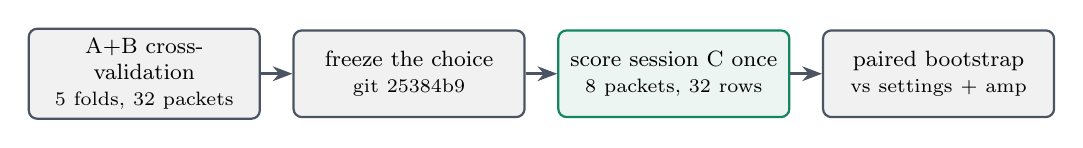
\begin{tikzpicture}[node distance=0.4cm]
\node[box,text width=2.7cm] (a) {A+B cross-validation\\\scriptsize 5 folds, 32 packets};
\node[box,right=of a,text width=2.7cm] (b) {freeze the choice\\\scriptsize git 25384b9};
\node[box=model,right=of b,text width=2.7cm] (c) {score session C once\\\scriptsize 8 packets, 32 rows};
\node[box,right=of c,text width=2.7cm] (d) {paired bootstrap\\\scriptsize vs settings + amp};
\foreach \x/\y in {a/b,b/c,c/d} \draw[arr] (\x)--(\y);
\end{tikzpicture}}
\end{center}
\end{frame}

% ============================================================================================================
\divider{Part 4}{First real data: can the traces predict the image?}{image!60}

\begin{frame}{The data were good enough to learn from}
\eyebrow[image]{The night of 2026-11-02}
\begin{columns}[T]
\column{0.24\textwidth}{\Huge\bfseries 43}\par\small packets, all at the right settings
\column{0.24\textwidth}{\Huge\bfseries\color{trace} 92\,\%}\par\small of board-101 traces usable
\column{0.24\textwidth}{\Huge\bfseries\color{image} 127}\par\small of 128 A+B labels usable
\column{0.24\textwidth}{\Huge\bfseries\color{problem} 3}\par\small C packets lost every trace
\end{columns}
\vspace{2em}
\begin{columns}[T]
\column{0.48\textwidth}\textbf{Training: sessions A + B}\par\small 32 packets, one knob at a time, 127 rows
\column{0.48\textwidth}\textbf{Test: session C}\par\small 8 usable packets, knobs changed together, 32 rows
\end{columns}
\end{frame}

\begin{frame}{On the held-out session, the physics model beats every baseline}
\eyebrow[image]{The headline}
\fig{0.62\textheight}{figures/fd_fig1_traces_help.png}
\begin{columns}[T]
\column{0.32\textwidth}\small\textbf{$\lambda$: 5.3\,\%} vs 23.2\,\% without a trace (significant)
\column{0.32\textwidth}\small\textbf{$\sigma_e$: 7.3\,\%} vs 10.2\,\% (not significant, 8 packets)
\column{0.32\textwidth}\small\textbf{gain: 0.9\,\%} vs 1.4\,\% (not significant)
\end{columns}
\end{frame}

\begin{frame}{Cross-validation on A+B did not rank the models the way session C did}
\eyebrow[image]{Every model}
\begin{columns}[c]
\column{0.66\textwidth}\fig{0.74\textheight}{figures/fd_fig7_all_models.png}
\column{0.32\textwidth}\small
$\circ$ A+B cross-validation \textperiodcentered{} $\bullet$ session C\par\medskip
Flexible models (gp\_dim, trees, nn) looked best in CV and fell back on C: A+B's one-knob packets made CV test \emph{extrapolation}.\par\medskip
physics (Allan floor) fails $\sigma_e$ at 29\,\%; physics\_white fixes it.
\end{columns}
\end{frame}

\begin{frame}{Session C, amplifier by amplifier}
\eyebrow[image]{Predicted vs true}
\begin{columns}[c]
\column{0.6\textwidth}\fig{0.76\textheight}{figures/fd_fig2_session_c.png}
\column{0.38\textwidth}\small
\textbf{Top:} the frozen choice; $\sigma_e$ scatters off the line.\par\medskip
\textbf{Bottom:} physics-structured; $\lambda$ follows the line across a factor of 3.\par\medskip
Band: $\pm$ the label scatter. Grey: A+B training rows.
\end{columns}
\end{frame}

\begin{frame}{Timing changes move the image's noise in ways the trace does not see}
\eyebrow[problem]{Where $\sigma_e$ goes wrong}
\begin{columns}[c]
\column{0.62\textwidth}\fig{0.36\textheight}{figures/fd_fig3_sigma_error_by_packet.png}\par\fig{0.36\textheight}{figures/fd_fig4_trace_vs_image.png}
\column{0.36\textwidth}\small
Session A (timing) is 43\,\% of the rows but \textbf{76\,\%} of the squared $\sigma_e$ error.\par\medskip
Voltage packets sit on the trace's noise line; timing packets scatter off it.\par\medskip
The trace reads 10 pixels after a 100-column burst; the image reads $10^4$ pixels after a 5300-column prescan and a clear.
\end{columns}
\end{frame}

\begin{frame}{Dark charge remembers the CCD's history}
\eyebrow[problem]{Where $\lambda$ goes wrong}
\begin{columns}[c]
\column{0.62\textwidth}\fig{0.6\textheight}{figures/fd_fig5_lambda_night.png}
\column{0.36\textwidth}\small
At fixed nominal settings $\lambda$ drifted down $\sim$20\,\% over the night.\par\medskip
Outliers near 00:50: \textbf{L1\_18}, whose queue stalled 38 min before the image with no flush.\par\medskip
v2 flushes right before every image and repeats nominal every 7 packets.
\end{columns}
\end{frame}

% ============================================================================================================
\divider{Part 5 \textperiodcentered{} 2026-11-04}{What did the models learn, and will it work on another CCD?}{model!60}

\begin{frame}{Shuffle one group of inputs, and see how far the prediction moves}
\eyebrow[model]{What each model relies on}
\begin{columns}[c]
\column{0.64\textwidth}\fig{0.74\textheight}{figures/fd_fig8_reliance.png}
\column{0.34\textwidth}\footnotesize
\[S_G=100\sqrt{\tfrac1n\textstyle\sum_i(\hat y_i^{(\pi_G)}-\hat y_i)^2}\,\%\]
\[L_G=\mathrm{err}_C^{(\pi_G)}-\mathrm{err}_C\]
$S$: what the model \emph{uses}; $L$: what \emph{helps} on new packets. Also shuffled \textbf{within each amplifier}: if that barely moves it, the group only says \emph{which amplifier}.
\end{columns}
\end{frame}

\begin{frame}{Most of the $\sigma_e$ accuracy comes from the measured noise itself}
\eyebrow[model]{Inside the physics model}
\fig{0.62\textheight}{figures/fd_fig9_physics_terms.png}
\begin{columns}[T]
\column{0.32\textwidth}\small\textbf{8.8\,\%} from $w/\sqrt N$ and the average gain alone
\column{0.32\textwidth}\small\textbf{7.6\,\%} with the learned gain
\column{0.32\textwidth}\small\textbf{7.3\,\%} with the correction (image $\approx0.82\times$ trace)
\end{columns}
\end{frame}

\begin{frame}{The reference trace mostly tells the model which amplifier it is looking at}
\eyebrow[problem]{Amplifier fingerprints}
\begin{columns}[c]
\column{0.66\textwidth}\fig{0.62\textheight}{figures/fig_fingerprint.png}
\column{0.32\textwidth}\small
\[\eta^2=1-\frac{\sum_a\sum_{i\in a}(x_i-\bar x_a)^2}{\sum_i(x_i-\bar x)^2}\]
the share of a feature's variance that is just ``which amplifier''.\par\medskip
\textbf{52} columns have $\eta^2>0.9$ (46 reference, 6 own). The own trace's noise features do not (white noise: 0.09).
\end{columns}
\end{frame}

\begin{frame}{On an amplifier it never saw, only the $\sigma_e$ physics model beats the average}
\eyebrow[model]{Leave one amplifier out}
\fig{0.6\textheight}{figures/fig_loao.png}
\begin{columns}[T]
\column{0.32\textwidth}\footnotesize\textbf{$\sigma_e$:} physics 12.3 $\to$ 14.0\,\% on a new amplifier; flexible models fall to the average (18.7\,\%)
\column{0.32\textwidth}\footnotesize\textbf{$\lambda$:} no model beats the average's level (55\,\%); after one image physics 28 vs 37\,\%
\column{0.32\textwidth}\footnotesize\textbf{gain:} nothing beats the average (3.5\,\%); after one image all $\approx$ 0.8--1\,\%
\end{columns}
\end{frame}

\begin{frame}{Without the fingerprints, $\lambda$ and gain get worse; $\sigma_e$ does not care}
\eyebrow[problem]{Removing the fingerprints}
\fig{0.6\textheight}{figures/fig_no_fingerprint.png}
\begin{columns}[T]
\column{0.32\textwidth}\footnotesize\textbf{$\lambda$:} physics 5.3 $\to$ 15.2\,\%; still better than settings + amplifier (23\,\%)
\column{0.32\textwidth}\footnotesize\textbf{gain:} physics 0.9 $\to$ 2.8\,\%: it came from recognising the amplifier
\column{0.32\textwidth}\footnotesize\textbf{$\sigma_e$:} physics 7.3 $\to$ 6.9\,\%: it never used them
\end{columns}
\end{frame}

\begin{frame}{Why recognising the amplifier is not predicting its gain}
\eyebrow[problem]{The gain}
\begin{columns}[T]
\column{0.5\textwidth}
\textbf{On known amplifiers} the model learns a lookup: ``ringing rms $\approx$ 12 ADU $\to$ ch0 $\to$ gain 1.34''.\par\medskip
\textbf{On a new amplifier} the fingerprint value has no gain attached, and 3 training amplifiers are 3 points: any curve fits them.
\column{0.46\textwidth}
\textbf{Physics:} the trace is in ADU and holds no known charge:
\[\sigma_1^{\rm ADU}=\sigma_e\times g\]
a quiet, high-gain amplifier looks like a noisy, low-gain one. Only whole electrons (the image's or a strip's peaks) separate them.
\end{columns}
\end{frame}

\begin{frame}{Trained on 101, tested on 102: levels miss, one image fixes them}
\eyebrow[problem]{Another module: board 102}
\begin{columns}[c]
\column{0.64\textwidth}\fig{0.5\textheight}{figures/fig_board102.png}
\column{0.34\textwidth}\small
$\sigma_e$: image/trace ratio 1.06 on 102 vs 0.82 on 101, so physics is 30\,\% low.\par\medskip
$\lambda$: 1.11 e$^-$/pixel, 2--4$\times$ board 101.\par\medskip
After one image: every model at the label scatter.
\end{columns}
\vspace{0.6em}
\colorbox{problem!10}{\parbox{0.95\textwidth}{\footnotesize\textbf{A weak test:} 102's settings never changed, ch0/1 are dead, ch3 is suspect, its $\sigma_e$ labels repeat only to 9--13\,\%. Used: ch2, 41 rows.}}
\end{frame}

\begin{frame}{Dropping 101 ch2 (EXT3) mainly helps $\lambda$ on unseen amplifiers}
\eyebrow[problem]{Without the noisy channel}
\begin{columns}[c]
\column{0.64\textwidth}\fig{0.74\textheight}{figures/fig_no_ch2.png}
\column{0.34\textwidth}\small
Scored on \textbf{ch0, ch1, ch3} only.\par\medskip
ch2: per-row fit $\chi^2$ 22 (others 3--4), $\lambda$ 0.61 (others 0.27--0.48).\par\medskip
\textbf{$\lambda$, new amplifier:} physics 70 $\to$ 49 $\to$ 46\,\%, nn 55 $\to$ 47 $\to$ 40\,\%: below the average (52\,\%) for the first time.\par\medskip
$\sigma_e$, gain: within the noise.
\end{columns}
\end{frame}

\begin{frame}{More packets still help $\sigma_e$ and $\lambda$}
\eyebrow[model]{Learning curve}
\fig{0.58\textheight}{figures/fig_learning_curve.png}\par
\small Trained on random subsets of A+B (5 draws per size), without ch2 and the fingerprints, scored on session C. physics $\sigma_e$ 9.7 $\to$ 5.9\,\%, $\lambda$ 19.0 $\to$ 10.4\,\% from 8 to 32 packets; the gain levels off near 1\,\%.
\end{frame}

\begin{frame}{Without the settings as input, nothing gets worse}
\eyebrow[model]{Traces only}
\small Every model trained without 101 ch2, without the fingerprints, and \textbf{with} vs \textbf{without} the 67 settings $\theta$ as input. Errors in \%, scored on ch0, ch1, ch3.\par\medskip
\begin{tabular}{lcccc}\toprule
 & \multicolumn{2}{c}{session C} & \multicolumn{2}{c}{new amplifier}\\
model, target & with $\theta$ & without $\theta$ & with $\theta$ & without $\theta$\\\midrule
physics, $\sigma_e$ & 5.9 & 6.1 & 14.4 & 14.9\\
cnn, $\sigma_e$ & 10.0 & 7.0 & 23.4 & 22.5\\
pretrained, $\sigma_e$ & 15.7 & \textbf{5.2} & 17.8 & 19.0\\
physics, $\lambda$ & 10.4 & 10.4 & 46.3 & 46.0\\
cnn, $\lambda$ & 13.2 & 11.8 & 44.4 & \textbf{39.7}\\
deep\_kernel, $\lambda$ & 20.3 & 17.5 & 53.2 & \textbf{42.0}\\
physics, gain & 2.0 & \textbf{0.7} & 3.6 & 3.7\\\bottomrule
\end{tabular}\par\medskip
The trace already carries what the models used the settings for. Traces-only models are simpler and do not learn a map of this CCD's knobs that would not carry to another CCD.
\end{frame}


\begin{frame}{Learn the changes; measure each amplifier's level once}
\eyebrow[model]{What carries to another CCD}
\[\log y(\theta,a)=c_a+f(\theta,\mathrm{trace}),\qquad c_a=\log y_{\rm measured}(\theta_0)-f(\theta_0)\]
\begin{columns}[T]
\column{0.32\textwidth}{\color{model}\bfseries $f$: learned}\par\small how the value moves with settings and the CCD's state
\column{0.32\textwidth}{\color{image}\bfseries $c_a$: measured}\par\small one number per amplifier and target, from one image or strip at nominal
\column{0.32\textwidth}{\color{trace}\bfseries how often}\par\small gain, $\sigma_e$ factor: stable (0.6\,\%, 2\,\%); $\lambda$ drifts 20\,\% a night
\end{columns}
\vspace{1em}
\small\textbf{The ideal model:} input = a trace at the settings to try + a one-time calibration per amplifier; output = the image's $\sigma_e$, $\lambda$, gain with error bars. Cost per try: seconds instead of $\sim$10 minutes.
\end{frame}

% ============================================================================================================
\divider{Part 6}{Next: better inputs, better data, a second CCD}{trace!60}

\begin{frame}{A tiny image read exactly like the real one, every skip kept}
\eyebrow{Level-1 strips}
\begin{columns}[T]
\column{0.5\textwidth}\small
$2\times1000$ pixels, 500 skips, after the same 5300-column prescan and clear as the image.\par\medskip
From it: the strip's own \textbf{gain} (peak spacing, $\sim$1\,\%), \textbf{CIC + serial charge} ($\sim$5\,\%), $\sigma_e$, white noise, Allan curve.\par\medskip
True dark current only weakly (strip rows barely wait): a second strip with a wait, or the image's rows.
\column{0.46\textwidth}
\resizebox{0.9\linewidth}{!}{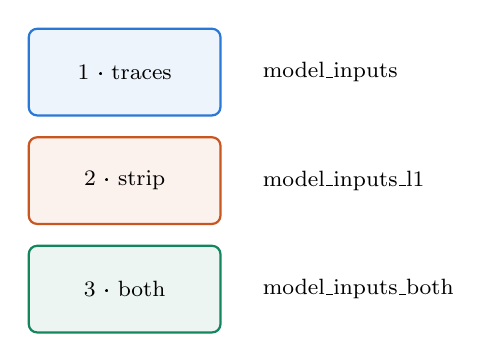
\begin{tikzpicture}[node distance=0.25cm]
\node[box=trace,text width=2.2cm] (a) {1 \textperiodcentered{} traces};
\node[box=image,below=of a,text width=2.2cm] (b) {2 \textperiodcentered{} strip};
\node[box=model,below=of b,text width=2.2cm] (c) {3 \textperiodcentered{} both};
\node[right=0.4cm of a,font=\footnotesize] {model\_inputs};
\node[right=0.4cm of b,font=\footnotesize] {model\_inputs\_l1};
\node[right=0.4cm of c,font=\footnotesize] {model\_inputs\_both};
\end{tikzpicture}}\par\medskip
\footnotesize Same rows, same folds: what do traces predict, what does the strip, and both?
\end{columns}
\end{frame}

\begin{frame}{Flushes, settle traces, strips and safeguards in every packet}
\eyebrow{The v2 packet}
\begin{center}
\resizebox{\textwidth}{!}{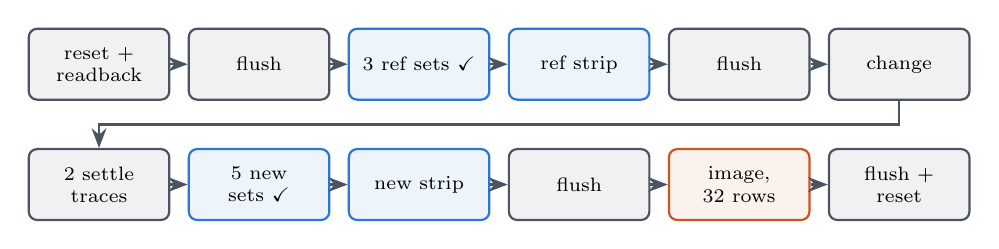
\begin{tikzpicture}[node distance=0.22cm]
\node[s] (a) {reset + readback}; \node[s,right=of a] (b) {flush};
\node[s=trace,right=of b] (c) {3 ref sets \checkmark}; \node[s=trace,right=of c] (d) {ref strip};
\node[s,right=of d] (e) {flush}; \node[s,right=of e] (f) {change};
\node[s,below=0.6cm of a] (g) {2 settle traces}; \node[s=trace,right=of g] (h) {5 new sets \checkmark};
\node[s=trace,right=of h] (i) {new strip}; \node[s,right=of i] (j) {flush};
\node[s=image,right=of j] (k) {image, 32 rows}; \node[s,right=of k] (l) {flush + reset};
\foreach \x/\y in {a/b,b/c,c/d,d/e,e/f,g/h,h/i,i/j,j/k,k/l} \draw[arr] (\x)--(\y);
\draw[arr] (f.south) -- ++(0,-0.3) -| (g.north);
\end{tikzpicture}}
\end{center}
\footnotesize\checkmark\ = checked on the spot; damaged traces retaken; more than 5 restarts the packet \textperiodcentered{} 2 s pause after every trace and image\par\medskip
\begin{columns}[T]
\column{0.32\textwidth}\small\textbf{76 packets, $\sim$21 h}\par\footnotesize session D (61) + session E (15, held out)
\column{0.32\textwidth}\small\textbf{Joint Sobol design}\par\footnotesize 12 knob groups move together
\column{0.32\textwidth}\small\textbf{Repeats}\par\footnotesize nominal every 7; 3 replicates
\end{columns}
\end{frame}

\begin{frame}{Next steps}
\eyebrow{From here to a model that works on any CCD}
\begin{columns}[T]
\column{0.32\textwidth}{\color{problem}\bfseries Before the v2 night}
\begin{itemize}\footnotesize
\item DAQ strip test: $1\times500$, $1\times1000$, $2\times1000$
\item pull main on the DAQ machine
\item change settings on \textbf{every working board}
\end{itemize}
\column{0.32\textwidth}{\color{trace}\bfseries After v2}
\begin{itemize}\footnotesize
\item traces vs strip vs both
\item train without ch2, fingerprints (and settings?)
\item choose on joint data, freeze, score session E once
\end{itemize}
\column{0.32\textwidth}{\color{model}\bfseries Later}
\begin{itemize}\footnotesize
\item train on one CCD, test on another
\item $\lambda$ formula: dark current $\times$ wait + CIC
\item level 2: safe Bayesian optimisation
\end{itemize}
\end{columns}
\end{frame}

{\setbeamercolor{background canvas}{bg=model}\setbeamertemplate{footline}{}
\begin{frame}[plain]
{\color{paper!80}\small\bfseries TAKEAWAYS}\par\vspace{0.6em}
{\color{paper}\Large\bfseries The trace measures $\sigma_e$; each amplifier's level must be measured once}\par\vspace{1.2em}
\color{paper}
\begin{columns}[T]
\column{0.48\textwidth}\small
\textbf{$\sigma_e$} transfers: read off the trace's white noise (7.3\,\% on C, 14\,\% on a new amplifier).\par\medskip
\textbf{Validation} must look like use: joint designs, prospective tests, new amplifiers, new CCDs.
\column{0.48\textwidth}\small
\textbf{$\lambda$ and gain} looked excellent on board 101, mostly by recognising the amplifier; a new one needs its level.\par\medskip
\textbf{v2 + strips}: inputs read like the image, a joint design, levels measured in every packet.
\end{columns}
\end{frame}}

\end{document}
